\documentclass[12pt,a4paper]{article}
\usepackage{amsmath,amsthm,amsfonts,amssymb,amscd}
\usepackage{times}
% Use Times New Roman
\usepackage{graphicx}
% Enhanced support for images
\usepackage{float}
% Improved interface for floating objects
\usepackage{booktabs}
% Publication quality tables
\usepackage{xcolor}
% Driver-independent color extensions
\usepackage{geometry}
% Customize document dimensions
\usepackage{fullpage}
% all 4 margins to be either 1 inch or 1.5 cm
\usepackage{comment}
% Commenting
\usepackage{minted}
% Highlighted source code. Syntax highlighting
\usepackage{listings}
% Typeset programs (programming code) within LaTeX
\usepackage{lastpage}
% Reference last page for Page N of M type footers.
\usepackage{fancyhdr}
% Control of page headers and footers
\usepackage{hyperref}
% Cross-referencing
\usepackage[small,bf]{caption}
% Captions
\usepackage{multicol}
\usepackage{tikz}
% Creating graphic elements
\usepackage{circuitikz}
% Creating circuits
\usepackage{verbatim}
% Print exactly what you type in
\usepackage{cite}
% Citation
\usepackage[us]{datetime}
% Various time format
\usepackage{blindtext}
% Generate blind text
\usepackage[utf8]{inputenc}
\usepackage{array}
\usepackage{makecell}
\usepackage{tabularx}
\usepackage{titlesec}

% \input {defs.tex}



\begin{document}

\textcolor{UM_Brown}{
% \begin{minipage}{0.1\textwidth}
%     \begin{flushleft}
%         \includegraphics[height=3.5cm]{UM_Logo_VERT_CMYK.eps}
%     \end{flushleft}
% \end{minipage}
\begin{minipage}{0.8\textwidth}
    \begin{center}
        \textbf{\Large Inference time of YOLOv5}\\
        \vspace{5pt}
        Team C \\
        \vspace{20pt}
        \textit{Sara Mohajerani} \\
        \vspace{5pt}
        \today
    \end{center}
\end{minipage}
\vspace{10pt}
\hrule
}



%%%%%%%%%%%%%%% NEW SECTION %%%%%%%%%%%%%%%
\section*{Inference time of GPU}
Here you can find the inference time of Yolov5s model on 470 images of kaggle data set, which selected as a test set in Fig. \ref{fig: gpu}. Fig. \ref{fig: gpu_hist} shows the histogram of these time.
\begin{figure}[H]
    \centering
    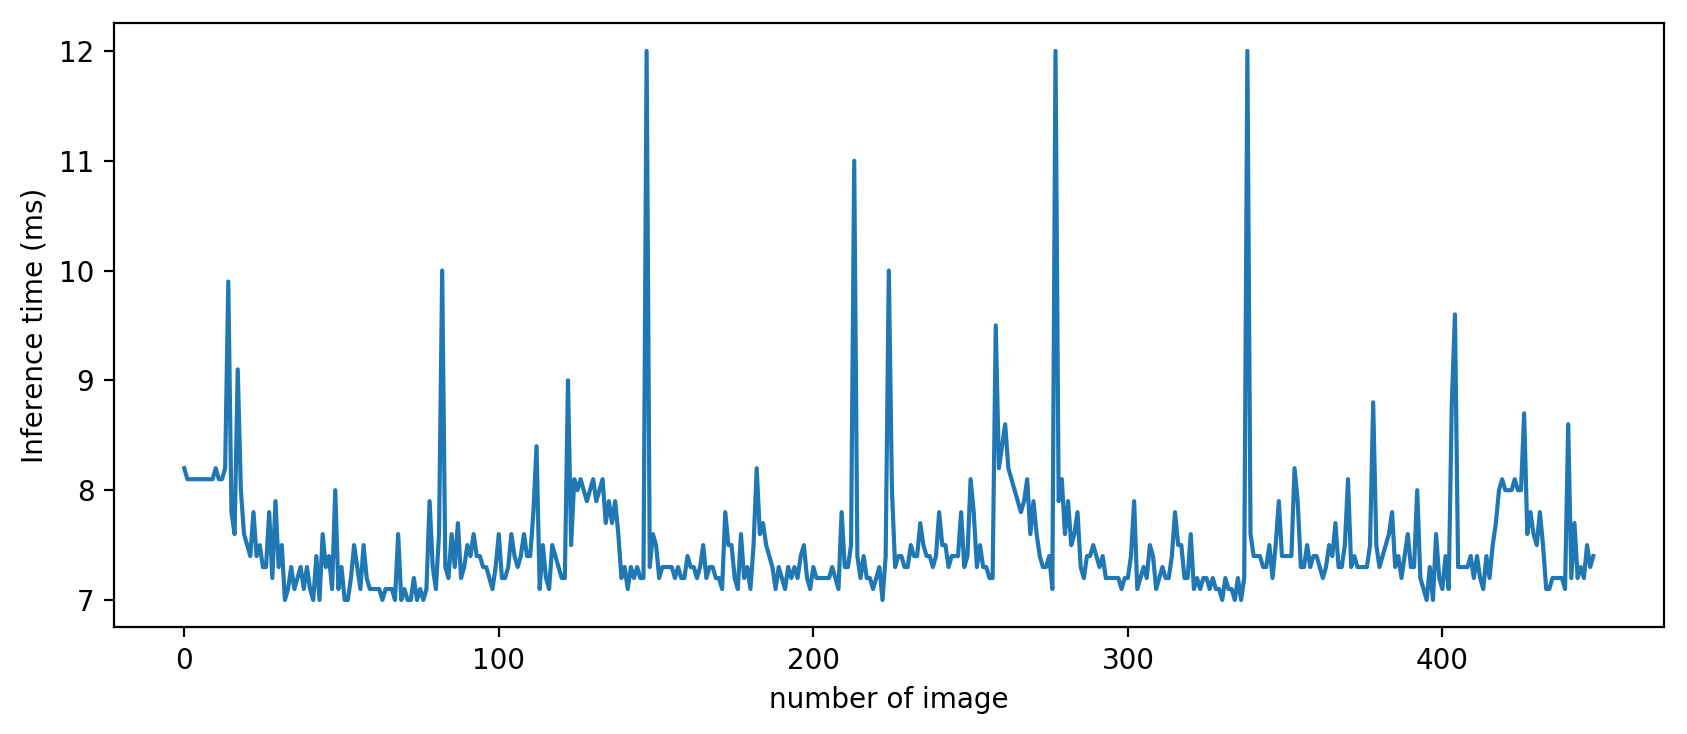
\includegraphics[width=15cm]{figures/GPU_infTime.png}
    \caption{The inference time of YOLOv5s model, when it run on GPU}
    \label{fig: gpu}
\end{figure}
\begin{figure}[H]
    \centering
    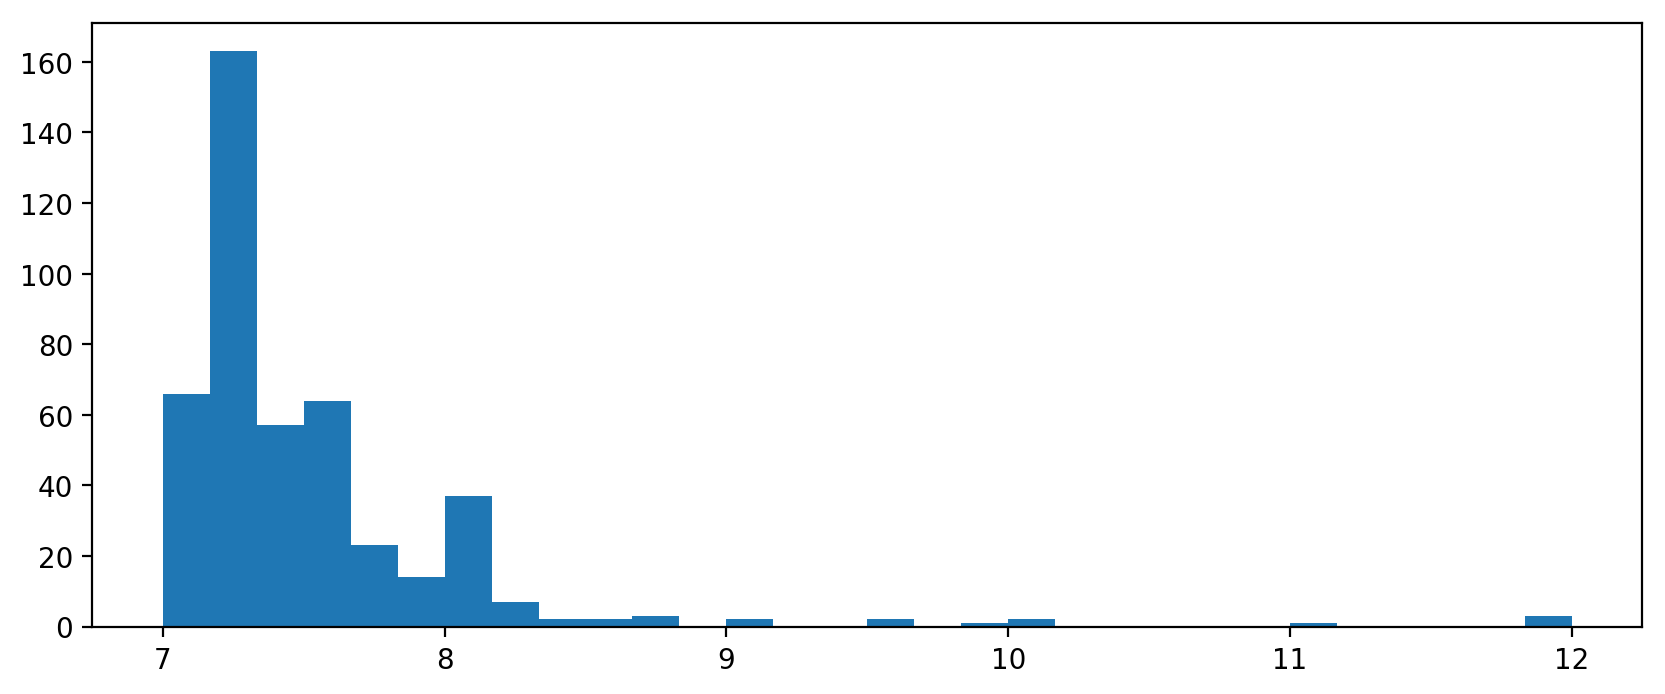
\includegraphics[width=15cm]{figures/GPU_infTime_his.png}
    \caption{The histogram of inference time of YOLOv5s model, when it run on GPU}
    \label{fig: gpu_hist}
\end{figure}
\subsubsection*{GPU pro}
Here the GPU model converted to the premium model. The inference time of YOLOv5s model on 470 images in test set of Kaggle data set is recorded and have been shown in Fig. \ref{fig: gpupro} and Fig. \ref{fig: gpupro_hist}.
\begin{figure}[H]
    \centering
    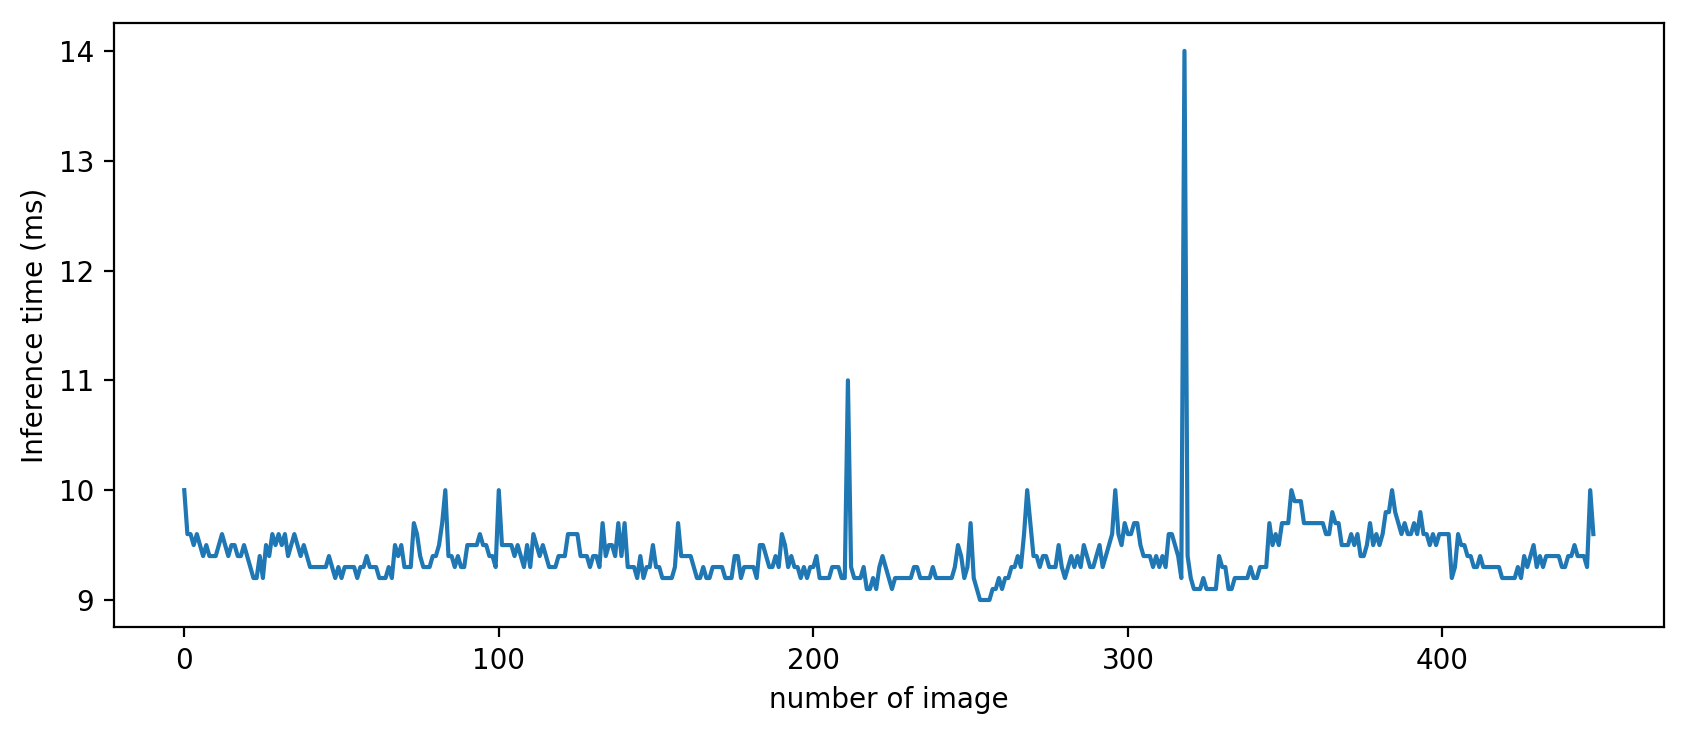
\includegraphics[width=15cm]{figures/gpupro.png}
    \caption{The inference time of YOLOv5s model, when it run on premium GPU}
    \label{fig: gpupro}
\end{figure}
\begin{figure}[H]
    \centering
    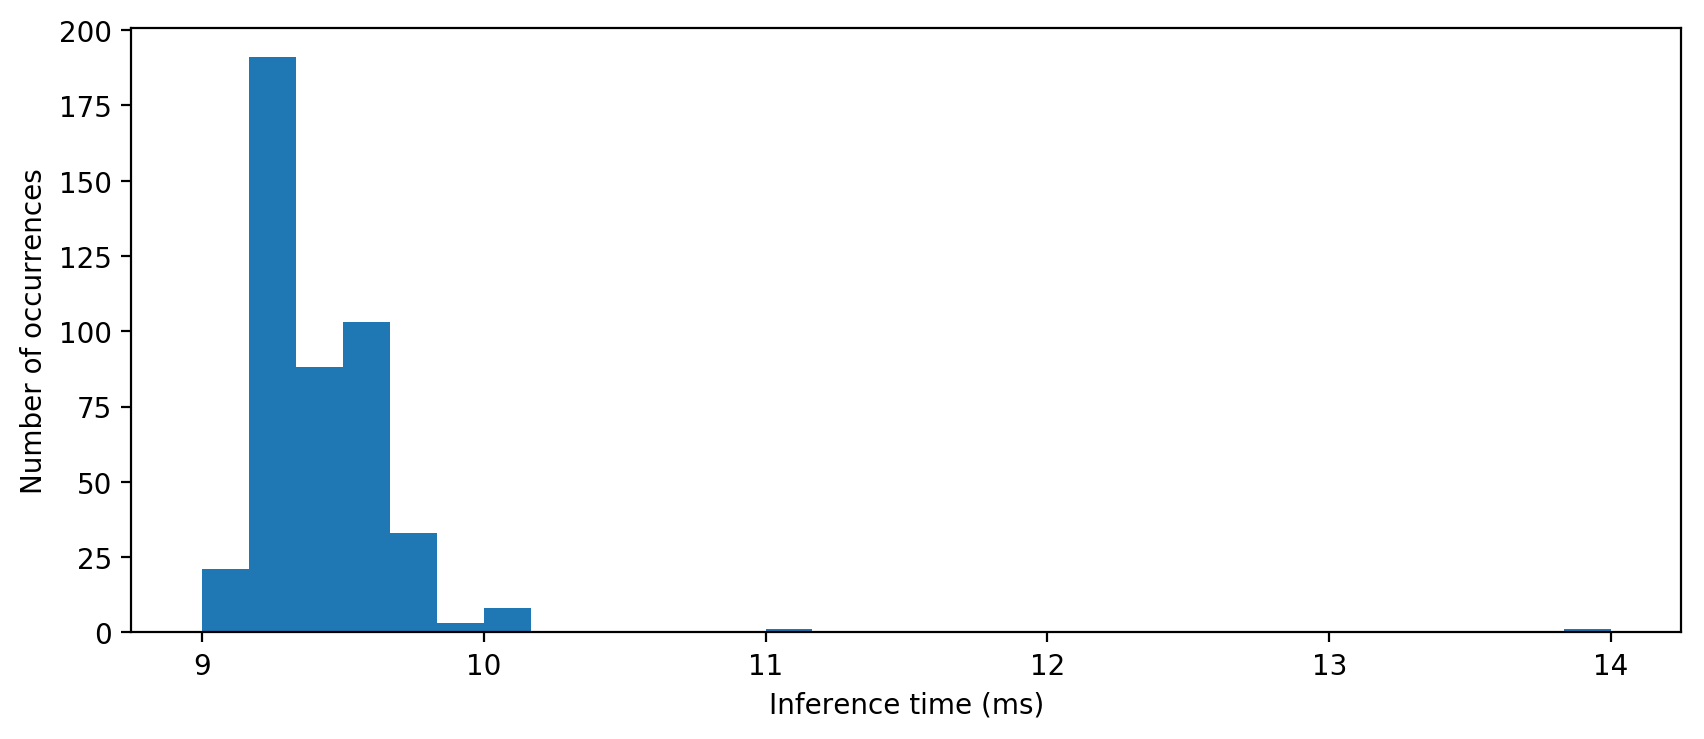
\includegraphics[width=15cm]{figures/gpupro_hist.png}
    \caption{The histogram of inference time of YOLOv5s model, when it run on premium GPU}
    \label{fig: gpupro_hist}
\end{figure}
The maximum inference time is equal to 14.0 ms. The minimum inference time is 9.0 ms and the standard deviation is 0.30. The total time is 4.224 s. In the second run the maximum inference time is equal to 20.0 ms. The minimum inference time is 8.8 ms and the standard deviation is 0.72. The total time is 4.149 s.
\subsection*{Half precision}
Here the GPU model converted to the premium model. The inference time of YOLOv5s model with half precision on 470 images in test set of Kaggle data set is recorded and have been shown in Fig. \ref{fig: gpuproh} and Fig. \ref{fig: gpuproh_hist}.
\begin{figure}[H]
    \centering
    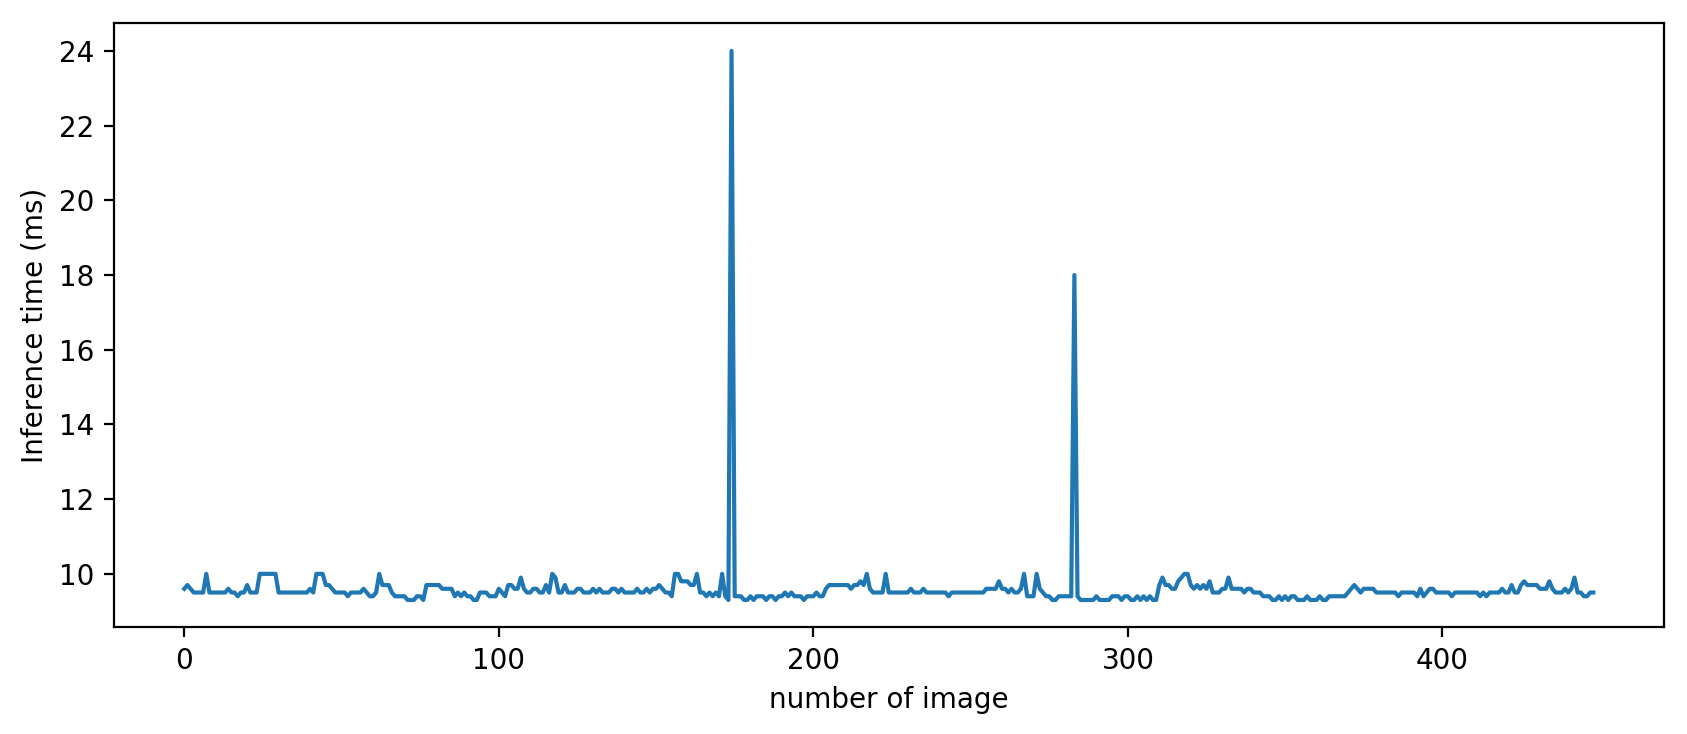
\includegraphics[width=15cm]{figures/proGPU_half.png}
    \caption{The inference time of YOLOv5s model, when it run on premium GPU with half precision}
    \label{fig: gpuproh}
\end{figure}
\begin{figure}[H]
    \centering
    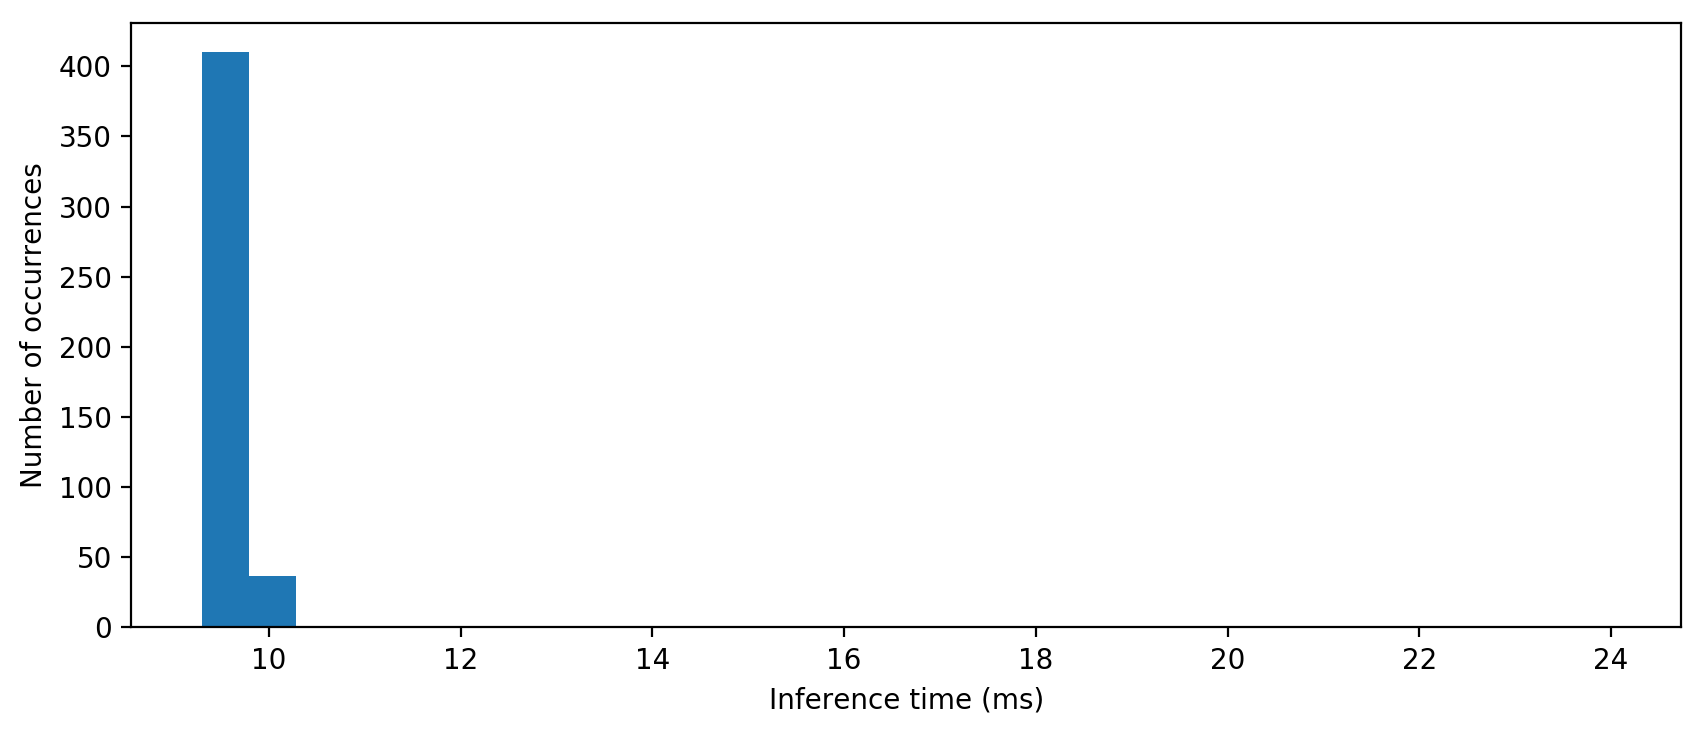
\includegraphics[width=15cm]{figures/proGPU_half_hist.png}
    \caption{The histogram of inference time of YOLOv5s model, when it run on premium GPU with half precision}
    \label{fig: gpuproh_hist}
\end{figure}
Here the inference time of Yolov5s model on 470 images of kaggle data set, with half precision is shown in Fig. \ref{fig: gpu_half}. Fig. \ref{fig: gpu_half_hist} shows the histogram of these recorded time.
\begin{figure}[H]
    \centering
    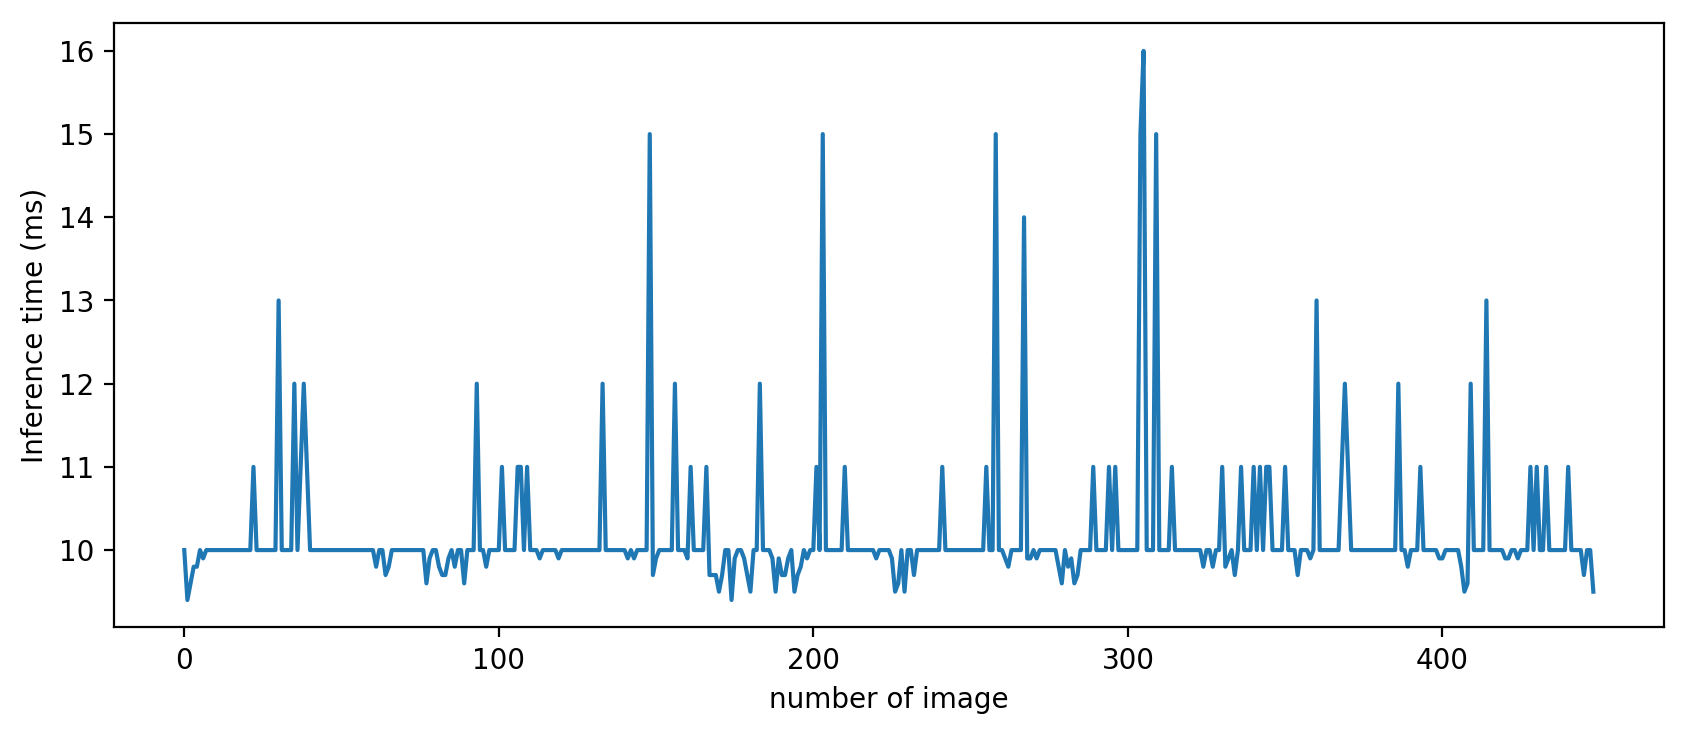
\includegraphics[width=15cm]{figures/GPU_infTime_half.png}
    \caption{The inference time of YOLOv5s model with half precision, when it run on GPU}
    \label{fig: gpu_half}
\end{figure}
\begin{figure}[H]
    \centering
    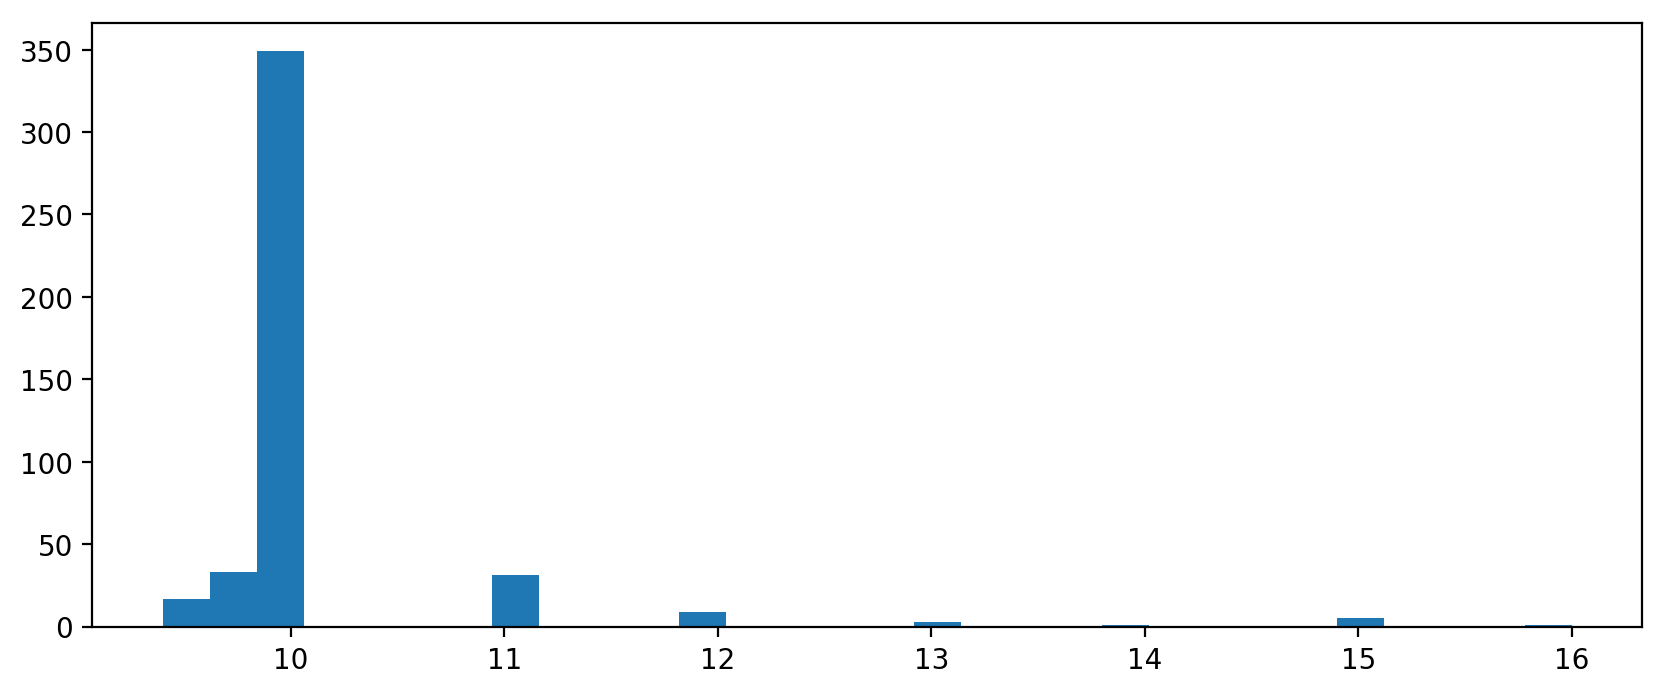
\includegraphics[width=15cm]{figures/GPU_infTime_half_hist.png}
    \caption{The histogram of inference time of YOLOv5s model with half precision, when it run on GPU}
    \label{fig: gpu_half_hist}
\end{figure}
\subsubsection*{GPU pro}
The maximum inference time is equal to 24.0 ms. The minimum inference time is 9.3 ms and the standard deviation is 0.81. The total time is 4.302 s. In the second run, we achieve the maximum inference time equal to 19.0 ms. The minimum inference time is 9.3 ms and the standard deviation is 0.59. The total time is 4.363 s.
%%%%%%%%%%%%%%% NEW SECTION %%%%%%%%%%%%%%%
\section*{Inference time of CPU}
Here you can find the inference time of Yolov5s model on 470 images of kaggle data set, which selected as a test set in Fig. \ref{fig: cpu}. Fig. \ref{fig: cpu_hist} shows the histogram of these time.
\begin{figure}[H]
    \centering
    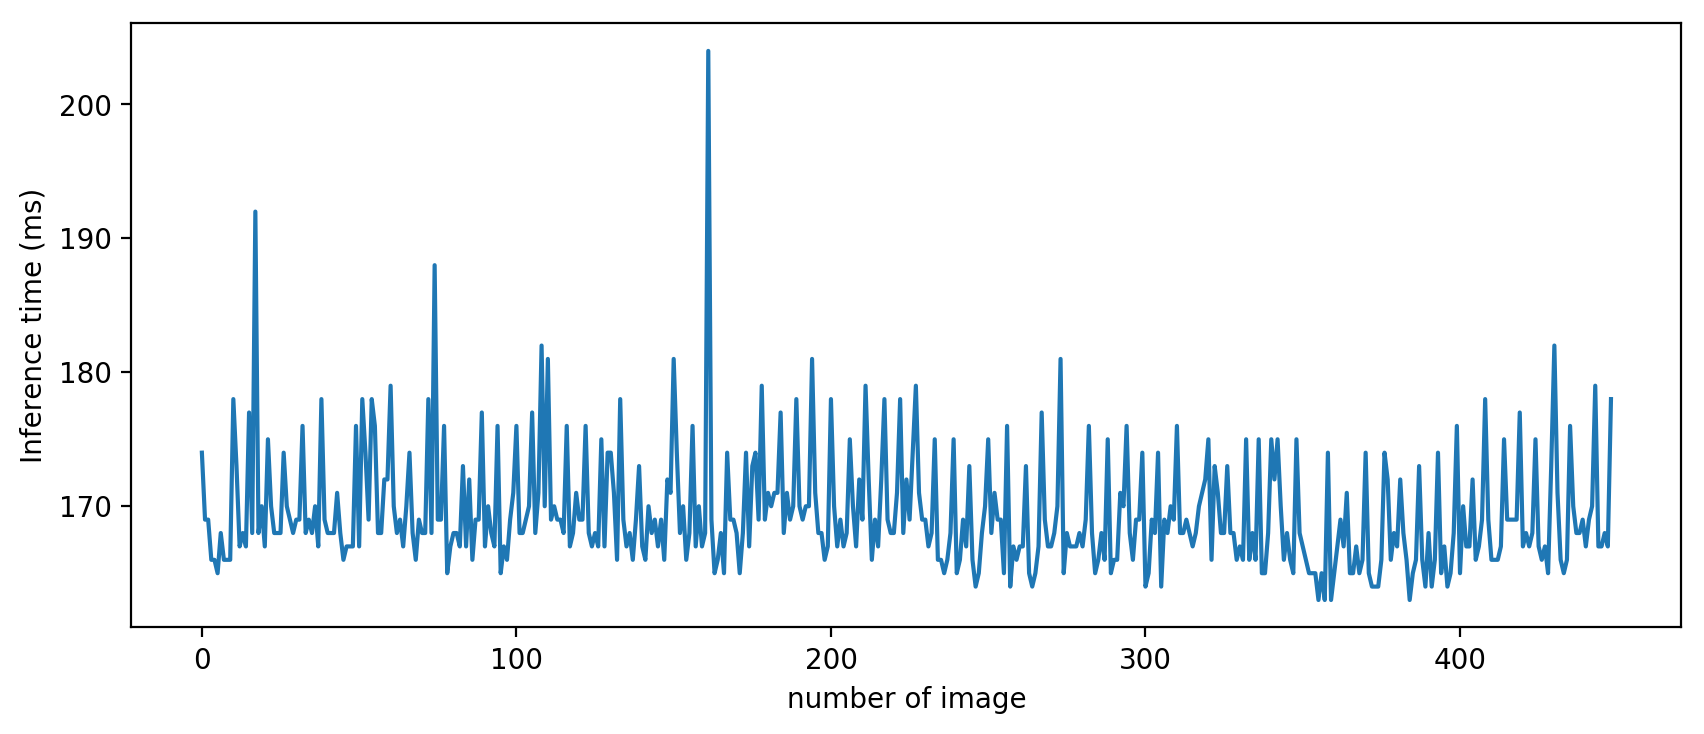
\includegraphics[width=15cm]{figures/CPU_infTime.png}
    \caption{The inference time of YOLOv5s model, when it run on CPU}
    \label{fig: cpu}
\end{figure}
\begin{figure}[H]
    \centering
    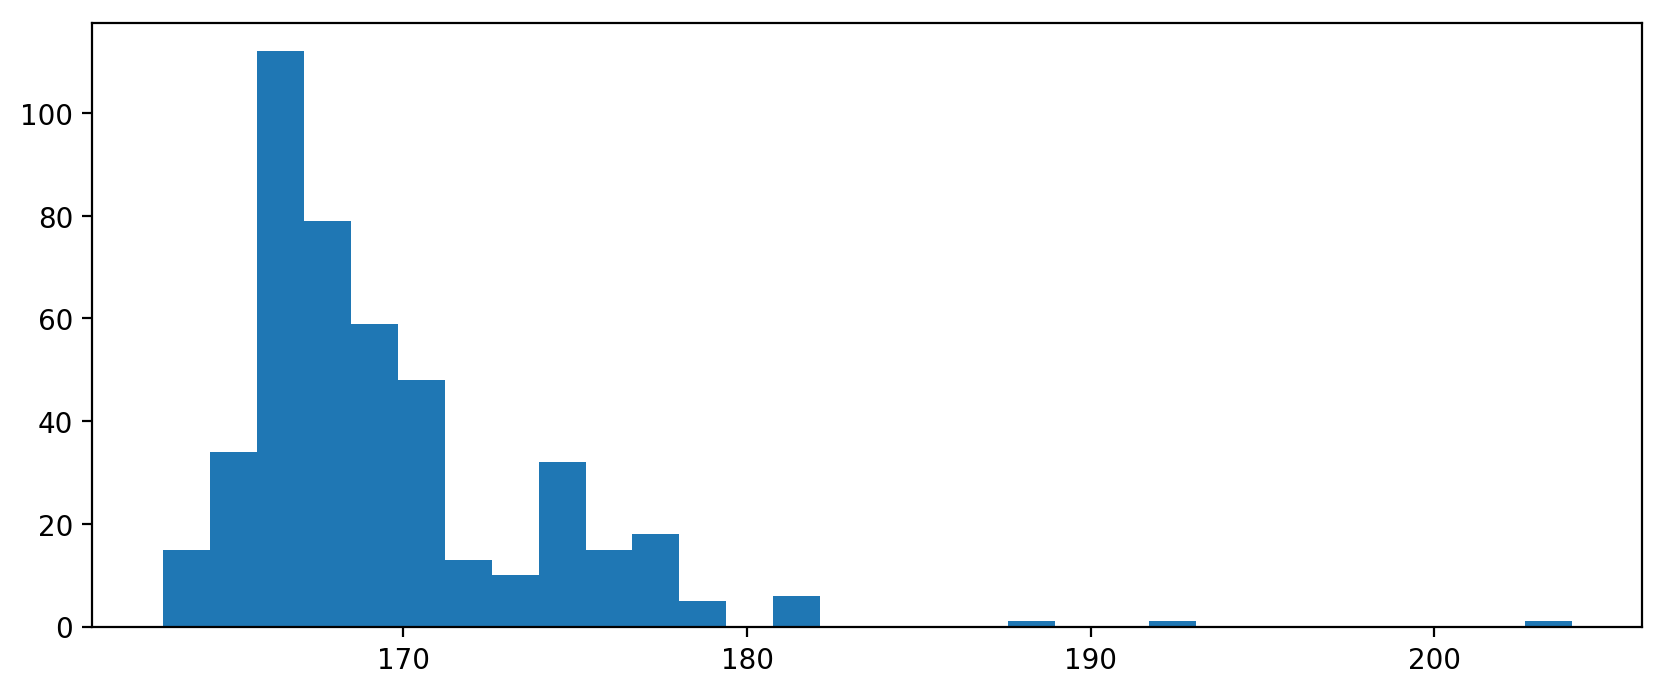
\includegraphics[width=15cm]{figures/CPU_infTime_hist.png}
    \caption{The histogram of inference time of YOLOv5s model, when it run on CPU}
    \label{fig: cpu_hist}
\end{figure}

%%%%%%%%%%%%%%% NEW SECTION %%%%%%%%%%%%%%%
\section*{Compare the results}

\begin{table}[H]
    \caption{The inference time with different scenarios}
    \label{tab: Data}
    \centering
    \begin{tabular}{c|c|c|c|c}
    \toprule
     \textbf{Name} &\bf{Min (ms)}& \bf{Max (ms)} & \textbf{Std} & \textbf{Total time (s)} \\
     \midrule
     GPU & 7 & 12 & 0.59 & 3.372\\
     GPU-half & 9.4 & 16 & 0.77 & 4.563 \\
     GPU(Pro) & 9 & 14 & 0.30 & 4.224\\
     GPU-half (Pro) & 9.3 & 24 & 0.81 & 4.302 \\
     CPU & 163 & 204 & 4.38 & 76.096  \\
     \bottomrule
    \end{tabular}
\end{table}



% %%%%%%%%%%%%%%% NEW SECTION %%%%%%%%%%%%%%%
% \section*{Problem 3: How to include graphics?}
% Images, figures, and photos are usually included in the context using the command \texttt{includegraphics}  inside \texttt{figure} environment.

% \begin{verbatim}
%     \begin{figure}[H]
%         \centering
%         \includegraphics[options]{filename}
%         \caption{caption for the figure}
%         \label{fig: figlabel}
%     \end{figure}
% \end{verbatim}

% Figure \ref{fig: ElemntsPE} shows some elements that are frequently used in power electronic converters. This figure is adopted from \cite{FPE}.

% \begin{figure}[H]
%     \centering
%     \includegraphics[width=15cm]{figures/elements.png}
%     \caption{Elements of power electronic converters}
%     \label{fig: ElemntsPE}
% \end{figure}

% For more information on how to use this package, please visit the following website: \\
% \url{https://latexref.xyz/_005cincludegraphics.html}



% %%%%%%%%%%%%%%% NEW SECTION %%%%%%%%%%%%%%%
% \section{Problem 4: How to cite?}
% Paper \cite{Gole97} provides guidelines for modeling power electronics in electric power engineering application. If you do not include any reference please delete the reference section at the end of the document (see three lines of code before \texttt{\textbackslash end\{document\}})









% %%%%%%%%%%%%%%% REFERENCES %%%%%%%%%%%%%%%
% \newpage
% \bibliographystyle{IEEEtran}
% \bibliography{References}








\end{document}
